\documentclass[../cnd.tex]{subfiles}

Khái niệm "Ethereum"$^{[4]}$ có thể được sử dụng để chỉ ba thứ khác nhau: giao thức Ethereum, mạng Ethereum, và dự án Ethereum bao gồm cả hai thứ trên. Có thể thấy sức mạnh chủ yếu của nó đến từ giao thức. 

 Ethereum là một nền tảng điện toán có tính chất phân tán, công cộng, mã nguồn mở dựa trên công nghệ Blockchain. Nó có tính năng Hợp đồng thông minh (Smart Contracts), tạo thuận lợi cho các thỏa thuận hợp đồng trực tuyến.
		
\subsubsection{Lịch sử ra đời}
Ethereum ban đầu được mô tả trong một văn bản của Vitalik Buterin, một lập trình viên liên quan đến Bitcoin vào cuối năm 2013 với mục tiêu xây dựng các ứng dụng phân quyền. Buterin đã lập luận rằng Bitcoin cần một ngôn ngữ kịch bản để phát triển ứng dụng. Không đạt được thỏa thuận với nhóm phát triển Bitcoin, ông đề xuất phát triển một nền tảng mới với một ngôn ngữ kịch bản tổng quát hơn.

%\begin{figure}[h]
%	\centering
%	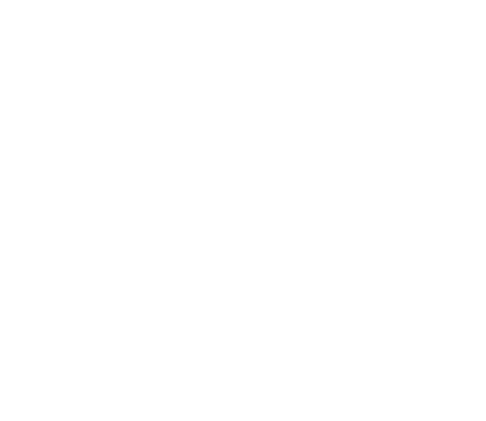
\includegraphics[width=0.7\linewidth]{C:/Users/kira/Desktop/logo}
%	\caption{Logo Ethereum}
%	\label{fig:ethereum-bw}
%\end{figure}

 Bốn thành viên ban đầu của nhóm Ethereum là Vitalik Buterin, Mihai Alisie, Anthony Di Iorio và Charles Hoskinson. Phát triển chính thức của dự án phần mềm Ethereum bắt đầu vào đầu năm 2014 thông qua một công ty Thụy Sĩ tên là Ethereum Switzerland GmbH (EthSuisse). Sau đó, một tổ chức phi lợi nhuận tại Thụy Sĩ với tên gọi là Ethereum Foundation cũng được thành lập. Việc phát triển Ethereum được tài trợ bởi đám đông trực tuyến trong suốt tháng 7 và tháng 8 năm 2014, với những người tham gia mua Ethereum bằng các loại tiền kỹ thuật số khác như bitcoin. Mặc dù đã có những lời khen ngợi đầu tiên về những đổi mới kỹ thuật của Ethereum, nhưng cũng có các ngờ vực về tính an toàn và khả năng mở rộng của nó 
		
\subsubsection{Các thành phần cơ bản của Ethereum $^{[5]}$} 
\paragraph{Ether}  
\indent

Tiền mã hóa được giao dịch trong mạng lưới Ethereum được gọi là ether. Nó được liệt kê dưới mã ETH và giao dịch trên các sàn giao dịch tiền mã hóa. Nó cũng được sử dụng để trả phí giao dịch và dịch vụ tính toán trên mạng Ethereum.

Đối với tiền ảo, thách thức để được chấp nhận vẫn còn tồn tại. Ngày nay, những token này vẫn là một lớp thanh toán nhanh, bảo mật và minh bạch nhất trong các hệ thống tiền tệ được công nhận đang tồn tại; Một sự triển khai thử nghiệm một ngày nào đó có thể thay thế các công nghệ mạng thanh toán tập trung như Visa hay Mastercard như ngày nay.

\paragraph{Gas}
\indent 

Gas là một đơn vị công việc được sử dụng để đo lường mức chi phí tính toán (computationally expensive) cho một giao dịch trên Ethereum có thể tiêu tốn. Giá trị của Gas được trả bằng một lượng nhỏ ether.
		
Có hai lý do chính để Gas được ra đời:
\begin{itemize}
	\item Thứ nhất, nó đảm bảo một phần thưởng được tả trước cho các thợ đào (miner) cho việc thực thi mã nguồn và bảo mật kết mạng, ngay cả khi việc thực thi bị thất bại vì một lý do nào đó. 
	\item Thứ hai, nó hoạt động xung quanh bài toán rừng và đảm bảo việc thực thi không thể dài quá thời gian đã được ước lượng trước đó.
\end{itemize}		

Gas là một đơn vị công việc, nó không phải là một đơn vị tiền tệ con, và bạn không thể sở hữu hay tích trữ nó. Nó chỉ đơn giản đo đạc mức tiêu hao mà hệ thống phải chịu nếu thực hiện giao dịch, ở mức các khái niệm tính toán. Để có thể trả chi phí Gas, bạn chỉ cần thêm ether vào tài khoản của bạn. Bạn không cần phải thu lấy nó một cách riêng biệt; không có khái niệm Gas token. Mọi toán tử trên EVM đều có một giá trị Gas nhất định.
	
Việc này khác so với ở Bitcoin, nơi mà chi phí được tính bằng kích thước của giao dịch tính bằng kilobytes, việc tính phí dựa trên khối lượng tính toán hợp lý hơn nhiều.

\paragraph{Máy ảo Ethereum (EVM)}
\indent 

Máy ảo Ethereum (EVM) là một môi trường chạy các hợp đồng thông minh Ethereum. Định nghĩa chính thức của EVM được quy định trong Ethereum Yellow Paper của Gavin Wood. Nó được hoàn toàn cô lập từ mạng, hệ thống tập tin và các quá trình khác của hệ thống máy chủ. Mỗi nút Ethereum trong mạng chạy một EVM và thực hiện các hướng dẫn giống nhau. Ethereum Virtual Machines đã được lập trình trong C++, Go, Haskell, Java, Python, Ruby, Rust và WebAssembly (hiện đang được phát triển)

\paragraph{Hợp đồng thông minh}
\indent 

Hợp đồng thông minh (smart contract) là một cơ chế trao đổi xác định, được kiểm soát bởi các phương tiện kỹ thuật số mà có thể giúp cho việc thực hiện giao dịch trực tiếp giữa các thực thể mà không cần tin cậy nhau. Các hợp đồng này được định nghĩa bằng cách lập trình và được chạy chính xác như mong muốn mà không bị kiểm duyệt, lừa đảo hay sự can thiệp từ bên thứ ba trung gian.
		
Chúng có thể được sử dụng để tạo điều kiện, xác minh và thực thi việc đàm phán hoặc thực hiện các hướng dẫn thủ tục kinh tế và có khả năng tránh được sự kiểm duyệt, thông đồng và rủi ro từ phía đối tác. Trong Ethereum, các hợp đồng thông minh được coi là các kịch bản tự trị hoặc các ứng dụng phân cấp được lưu trữ trong chuỗi khối Ethereum để thực hiện sau đó bởi EVM. Các hướng dẫn được nhúng trong các hợp đồng Ethereum được thanh toán bằng ether và có thể được thực hiện bằng nhiều ngôn ngữ Turing-complete khác nhau.

Sự khác biệt giữa hợp đồng truyền thống và hợp đồng hiện đại:
\begin{itemize}
	\item Hợp đồng truyền thống được tạo bởi các chuyên gia pháp lí để biên soạn và thực thi. Điều này rất mất thời gian và không minh bạch. Hợp đồng có sự cố sảy ra thì phải dựa vào hệ thống pháp lí giải quyết và điều này tốn các chi phí liên quan.
	\item Hợp đồng thông minh được tạo ra bởi hệ thống máy tính bằng ngôn ngữ lập trình. Trong đó nêu rõ các điều khoản và hình phạt tương đương với các hợp đồng truyền thống đưa ra. Nhưng hợp đồng thông minh không cần sự can thiệp của con người, do đó đảm bảo việc thự thi hợp đồng được chính xác và công minh nhất. Toàn bộ đoàn mã của hợp đồng thông minh được thực hiện bởi hệ thống sổ cái phân tán chuỗi khối.			
\end{itemize}

\paragraph{Solidity}
\indent 
		
Solidity là một ngôn ngữ lập trình sử dụng để viết các chương trình được gọi là hợp đồng thông minh (smart contract), thứ mà sẽ được chạy trên EVM. Ngôn ngữ mới này là một sự pha trộn các công ước từ mạng, hợp ngữ (assembly language) và phát triển web. Solidity là một ngôn ngữ cấp cao có định hướng hợp đồng, có cú pháp tương tự như của JavaScript và nó được thiết kế để nhắm mục tiêu Ethereum Virtual Machine (EVM).

Solidity là ngôn ngữ bậc cao được biên dịch bằng bytecode và được đưa lên chuỗi khối Ethereum bằng cách dùng các phần mềm phía người dùng như trình duyệt Mist hoặc nút (node). Ngôn ngữ Solidity định kiểu mạnh, hỗ trợ thừa kế, thư viện và các loại người dùng xác định  và phức tạp giữa các tính năng khác.

Solidity có khả năng thể hiện tất cả các nhiệm vụ có thể thực hiện được bằng máy tính, làm cho chúng về mặt lý thuyết là Turing hoàn chỉnh. Điều đó có nghĩa là toàn bộ mạng phân phối, mỗi nút, thực hiện mọi chương trình được thực hiện trên nền tảng này. Khi một người dùng tải lên một hợp đồng thông minh thông qua nút Ethereum của họ, nó được bao gồm trong khối mới nhất và được truyền bá xung quanh mạng, nơi nó được lưu trữ trên mọi nút khác trong mạng.

\paragraph{Decenterlized App}
\indent 

Decenterlize App (DAPP) là ứng dụng mã nguồn mở hoàn chỉnh, hoạt động độc lập, không có thực thể nào kiểm soát phần lớn các tokens của ứng dụng này và dữ liệu và hồ sơ hoạt động của ứng dụng phải được lưu trữ dưới dạng mã hoá công khai, phân quyền chuỗi khối.

Ứng dụng này tạo các mã thông báo theo một thuật toán tiêu chuẩn hoặc bộ tiêu chuẩn và có thể phân phối một số hoặc tất cả các tokens của nó khi bắt đầu hoạt động. Các tokens này phải là cần thiết cho việc sử dụng ứng dụng và bất kỳ đóng góp nào từ người dùng sẽ được thưởng bằng các khoản thanh toán trong các tokens của ứng dụng. Ứng dụng có thể thích ứng các giao thức của nó để đáp ứng với những cải tiến đề xuất và phản hồi thị trường nhưng tất cả thay đổi phải được quyết định bởi sự đồng thuận của người sử dụng. DAPP có giá trị và có khả năng phá vỡ một số ngành công nghiệp.

Phân loại DAPP:
\begin{itemize}
	\item Các ứng dụng phân cấp có chuỗi khối riêng như bitcoin.
	\item Giống như loại 1 nhưng có thêm token và các giao thức cần thiết như giao thức omni
	\item Giống như loại 2 nhưng có các mã thông báo cần thiết
\end{itemize}
		
Lợi ích của DAPP:
\begin{itemize}
	\item The Safe Network: có sự bảo mật lớn nhất
	\item Factom: đơn giản hóa quá trình tăng cường quá trình ghi lại quá trình quản lý dữ liệu lớn
	\item BURST: giải quyết các vấn đề đã làm lưu trữ đám mây đắt đỏ và không đáng tin cậy
	\item Augur: được biết đến như là một thị trường dự đoán phân quyền để thưởng cho người sử dụng về các sự kiện dự báo
	\item BlockAuth: cung cấp một hệ thống đa chữ ký để chia sẻ dữ liệu cá nhân với các bên thứ ba
\end{itemize}
		
\paragraph{Giao thức GHOST (Greedy Heaviest Observed Subtree)}
\indent 

"Grey Heaviest Observed Subtree" (GHOST) là một cải tiến được giới thiệu lần đầu tiên vào tháng 12 năm 2013. Động lực đằng sau GHOST ra đời đó là thời gian xác nhận các chuỗi khối nhanh chóng hiện đang phải chịu sự giảm an ninh do tỷ lệ lỗi cao - bởi vì các khối mất một thời gian nhất định để truyền thông qua mạng.

Nếu thợ đào mỏ A khai thác một khối và sau đó thợ đào mỏ B tình cờ đào mỏ khác trước khi khối của thợ mỏ A truyền cho B, khối thợ mỏ B đào sẽ kết thúc, bị lãng phí và không đóng góp cho an ninh mạng. Hơn nữa, có một vấn đề tập trung hóa: nếu thợ mỏ A là một mỏ khai thác với 30\% năng lượng (hashpower) và B có 10\% năng lượng, A sẽ có nguy cơ tạo ra một khối cũ 70\% thời gian (do đó 30\% thời gian khác A sản xuất khối cuối cùng và vì vậy sẽ lấy được dữ liệu khai thác được ngay lập tức) trong khi B sẽ có nguy cơ sản xuất một khối thời gian 90\% thời gian. Do đó, nếu khoảng thời gian là đủ ngắn cho tỷ lệ khối cũ để được cao, A sẽ được hiệu quả hơn rất nhiều chỉ đơn giản bởi hiệu quả của kích thước của nó.

Với hai hiệu ứng kết hợp, các chuỗi khối sản xuất khối một cách nhanh chóng rất có thể dẫn đến một mở chứa có một tỷ lệ phần trăm đủ lớn của mạng lưới hashpower để kiểm soát quá trình khai thác trong thực tế. Như được mô tả, GHOST giải quyết vấn đề đầu tiên của mất mát an ninh mạng bằng cách bao gồm các khối cũ trong việc tính chuỗi nào là "dài nhất"; có nghĩa là không chỉ là cha mẹ và các tổ tiên khác của một khối, mà còn là hậu duệ cũ của tổ tiên của khối (trong thuật ngữ Ethereum, "Uncle" (bác)) được thêm vào để tính khối mà có tổng số bằng chứng của sự hỗ trợ công việc lớn nhất. Để giải quyết vấn đề thứ hai về xu hướng tập trung, chúng ta vượt qua các giao thức được mô tả, và cũng cung cấp các phần thưởng block cho các stales: một khối cũ nhận được 87,5\% phần thưởng cơ bản của nó, và con cháu (nephew) có khối cũ nhận được 12,5\% phần thưởng còn lại. Tuy nhiên, phí giao dịch không được thưởng cho Uncle.

Phiên bản Ethereum của Ghost chỉ rơi vào bảy cấp độ - hoặc trở lại bảy cấp độ trong chiều cao của chuỗi khối:
\begin{itemize}
	\item Một khối phải chỉ định cha mẹ, và nó phải chỉ định 0 hoặc nhiều Uncle
	\item Đối với mỗi Uncle U trong khối B, thợ mỏ B được cộng thêm 3,125\% vào phần thưởng coinbase và người thợ mỏ của U được 93,75\% của phần thưởng coinbase tiêu chuẩn.
	\item Một Uncle bao gồm trong khối B phải có các tính chất sau:
		\begin{itemize}
			\item Nó phải là con trực tiếp của tổ tiên thế hệ k của B, trong đó 2 <= k <= 7
			\item Nó không thể là tổ tiên của B
			\item Một Uncle phải có tiêu đề khối hợp lệ, nhưng trước đó không cần xác minh hay thậm chí là một khối hợp lệ
			\item Một Uncle phải khác mọi Uncle khác bao gồm trong các khối trước và tất cả những Uncle khác nằm trong cùng một khối (không bao gồm hai lần)
		\end{itemize}
\end{itemize}